\begin{frame}
  \vfill
  {\LARGE
    \begin{center}
      BACKUP SLIDES
    \end{center}
  }
  \vfill
\end{frame}

\begin{frame}%

  {\small%
    \textbf{Argument against viscosity - viscous length scales}\\
    $\nu_{w}=0.7$ $\mu$m$^2$/s,\qquad
    $\nu_{a}=16.6 \mu$m$^2$/s,\qquad
    $f_c=\orderof{10^6}$Hz\\
    $\sqrt{\nu_{air}/f_c}=4\mu$ m $=\orderof{10^{-6}} << L_{\text{alveolus}}=\orderof{10^{-4}}$\\ \vspace*{4pt}
    $\sqrt{\nu_{air,ND}t} \approx0.5 < a(t)-a_0\approx4$ at $t=1000$\\ \vspace*{4pt}  
    Therefore the scale of the viscous effect is smaller than the scale of the problem we are looking at, but may be important at late times.\\
  }    
  % 
  \vspace*{0.25cm}
  \textbf{{\small Dimensional Numbers}}
  {\small
    \begin{itemize}
    \item Let $\lambda_{alveolus}=100 \mu$ m, $u_0=c_{air}=343$ m, $v_0=<\dot{a(t)}>\approx0.65$ m/s, $u_{intf}(t=20)=12.8$ m/s, $G=1$ kPa %\cite{Roan2011}
    \item $\lambda_{alveolus}=100 \mu$ m, $u_0=c_{air}=343$ m, $v_0=<\dot{a(t)}>\approx0.65$ m/s
    \item $t=1 \rightarrow t_{dim}=0.292 \mu$ s
    \end{itemize}
  }
  % 
  \vspace*{0.25cm}
  \textbf{{\small Dimensionless Numbers}}
  {\small
    \begin{itemize}
    \item $Fr=\frac{u_0}{\sqrt{g_0 \lambda}}\approx11000$
    \item $Fr=\frac{v_0}{\sqrt{g_0 \lambda}}\approx21$
    \item $Ca=\frac{\rho u_{intf}^2}{G_{Alv}} = 163$
    \end{itemize}
  }
  % 
\end{frame}

\begin{frame}\frametitle{\vspace*{0.5cm}Interface treatment}
  {\small
    \begin{minipage}{0.55\textwidth}
      Interface thickness parameter:
      \begin{align*}
        \delta = 0.08\lambda%
      \end{align*}
      
      Normalized distance from interface:
      \begin{align*}
        d = \frac{\delta +y(x)_{interface} -y}{2\delta}
      \end{align*}


      Volume fraction:%
      \begin{align*}
        y_0 = %
        \begin{cases}
          1\\%
          exp\left(log\left(10^{-16}\right)\abs{d}^8\right)\\%
          0%
        \end{cases}%
      \end{align*}
    \end{minipage}
    % 
    \begin{minipage}{0.4\textwidth}
      \begin{figure}
        \centering
        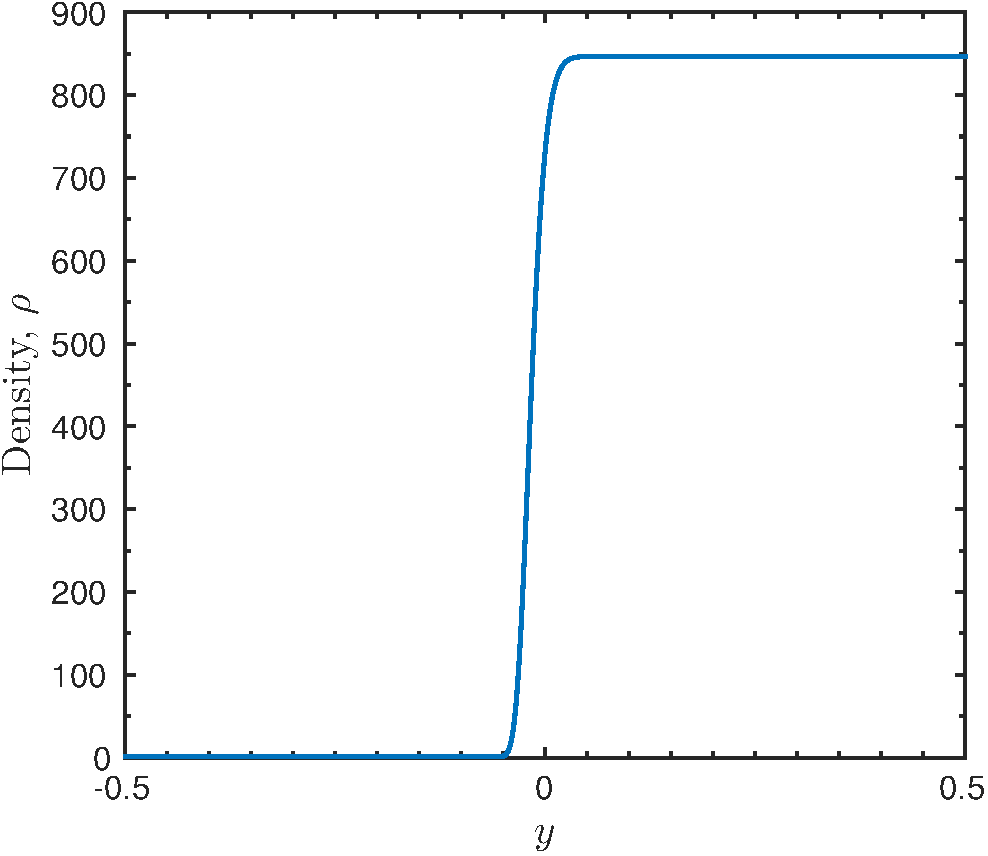
\includegraphics[width=\textwidth]{./figs/interface_density}
      \end{figure}
    \end{minipage}
  }
  % 
\end{frame}

\begin{frame}\frametitle{Radiation Pressure}
  $P_{net}=\frac{\Delta p_a}{2}\left[1-\frac{c_w}{c_a}+\frac{(\rho c)_a-(\rho c)_w}{(\rho c)_a(\rho c)_w}\right]$ \cite{Beyer1974}
  

  Stress failure in the lungs:\\
  Rabbit lungs under transmural pressure: $\approx 5.2 kPa$ \citep{West1991};

  
  
  
\end{frame}


%%% Local Variables:
%%% mode: latex
%%% TeX-master: "../main"
%%% End:
